% **************************************************************************************************************
% A Classic Thesis Style
% An Homage to The Elements of Typographic Style
%
% Copyright (C) 2015 André Miede http://www.miede.de
%
% If you like the style then I would appreciate a postcard. My address 
% can be found in the file ClassicThesis.pdf. A collection of the 
% postcards I received so far is available online at 
% http://postcards.miede.de
%
% License:
% This program is free software; you can redistribute it and/or modify
% it under the terms of the GNU General Public License as published by
% the Free Software Foundation; either version 2 of the License, or
% (at your option) any later version.
%
% This program is distributed in the hope that it will be useful,
% but WITHOUT ANY WARRANTY; without even the implied warranty of
% MERCHANTABILITY or FITNESS FOR A PARTICULAR PURPOSE.  See the
% GNU General Public License for more details.
%
% You should have received a copy of the GNU General Public License
% along with this program; see the file COPYING.  If not, write to
% the Free Software Foundation, Inc., 59 Temple Place - Suite 330,
% Boston, MA 02111-1307, USA.
%
% **************************************************************************************************************
\RequirePackage{fix-cm} % fix some latex issues see: http://texdoc.net/texmf-dist/doc/latex/base/fixltx2e.pdf
\documentclass[ twoside,openright,titlepage,numbers=noenddot,headinclude,%1headlines,% letterpaper a4paper
                footinclude=true,cleardoublepage=empty,abstractoff, % <--- obsolete, remove (todo)
                BCOR=5mm,paper=a4,fontsize=11pt,%11pt,a4paper,%
                ngerman,american,%
                ]{scrreprt}

%********************************************************************
% Note: Make all your adjustments in here
%*******************************************************
\input{classicthesis-config}

%********************************************************************
% Bibliographies
%*******************************************************
\addbibresource{Bibliography.bib}
\addbibresource[label=ownpubs]{AMiede_Publications.bib}

%********************************************************************
% Hyphenation
%*******************************************************
%\hyphenation{put special hyphenation here}

% ********************************************************************
% GO!GO!GO! MOVE IT!
%*******************************************************
\begin{document}
\frenchspacing
\raggedbottom
\selectlanguage{american} % american ngerman
%\renewcommand*{\bibname}{new name}
%\setbibpreamble{}
\pagenumbering{roman}
\pagestyle{plain}
%********************************************************************
% Frontmatter
%*******************************************************
%*******************************************************
% Little Dirty Titlepage
%*******************************************************
\thispagestyle{empty}
%\pdfbookmark[1]{Titel}{title}
%*******************************************************
\vspace*{\fill}\noindent{%\rule{\linewidth}{1mm}\\[4ex]
{\Huge \spacedallcaps \myTitle\\}\\[1ex]
{\large \spacedallcaps \mySubtitle}\\[4ex]
{\Large \spacedlowsmallcaps \myName, \myStudentId }\\[1ex]
{\Large \spacedlowsmallcaps \myNametwo, \myStudentIdtwo }\\[1ex]
\noindent\rule{\linewidth}{1mm}\\[4ex]
\noindent{\large \spacedlowsmallcaps \myDegree\\[1ex] 
\monthname\ \the\year  \\[1ex] Advisor: \myProf \\[23ex]}\\[\fill]}
\includegraphics[width=\linewidth]{gfx/logo}\clearpage


\include{FrontBackmatter/Titlepage}
\include{FrontBackmatter/Titleback}
\cleardoublepage\include{FrontBackmatter/Dedication}
%\cleardoublepage\include{FrontBackmatter/Foreword}
\cleardoublepage\include{FrontBackmatter/Abstract}
%\cleardoublepage\include{FrontBackmatter/Publications}
%\cleardoublepage\include{FrontBackmatter/Acknowledgments}
\pagestyle{scrheadings}
\cleardoublepage\include{FrontBackmatter/Contents}
%********************************************************************
% Mainmatter
%*******************************************************
\cleardoublepage\pagenumbering{arabic}
%\setcounter{page}{90}
% use \cleardoublepage here to avoid problems with pdfbookmark
\cleardoublepage
% What should a thesis contain:

\ctparttext{The following reflects what I believe to be a good structure
  for a report or a thesis in experimental computer science. 
It contains a natural progression from the general to the specific, and
from the work of others to the work by the authors, each chapter
forming the foundation of the next.}
\part{The Proper Structure of a Thesis}
\label{part:prop-struct-thes}
\cleardoublepage

\chapter{Introduction}\label{cha:introduction}
Today we have a lot of different chat systems used for different purposes. These chat systems are build for all kind of operating systems. 
Some of which are not encrypted, others are client-side encrypted and a few are end-to-end encrypted. Common for most of these chat systems are the dependency on centralized solutions which sort of can have some back doors that can create uncertainty about privacy of data. 

Peer-to-Peer (P2P) which is a decentralized way of communicating is an architecture where no one can have a superior role opposed to e.g. a client/server solution or other solutions with third-party interactions. By using P2P one gets rid of the uncertainty for others knowing about data or communication that is meant to be private. 

P2P could be a good alternative for an infrastructure used for chat systems. There already exist designs and implementations of P2P based chat systems e.g. SCRIBE. None of these solutions can catch up with today's existing popular client/server based chat systems. 

This project is intended to build a confidential and fair group chat system based on Kademlia.

%The purpose of the Introduction is make a short (2--6 pages) argument
%that should cover
%\begin{itemize}
%\item What this thesis is about
%\item Why it is interesting or important
%\item What are the central hypotheses that will be investigated 
%\item How will the work be done
%\end{itemize}
%
%This is the place where the reader (who will be a computer scientist,
%but might not be a domain expert) should be convinced that not only is
%the topic interesting and important, the authors have also identified
%central questions/hypotheses pertaining the topic, and have a clear
%plan and methodology to address it.
%
%\section{What makes a good hypothesis?}
%\label{sec:what-makes-good}
%
%For the purposes of a report or thesis, it is wise to concentrate on
%research questions and hypotheses that are quantifiable. \Eg, it is
%better to state that ``method A is better than method B under
%circumstances C'' or ``combining method A with architecture B improves
%on standard approach C'' than ``we can build a system that do X''.
%This is why it is always a good idea to include baselines in your
%work, \ie, established methods or architectural choices that can used
%for comparison. If you do not have baselines yourself, you should at
%least be ready and able to compare your results with the published
%results of others.
%
%The hypotheses should also address central aspects of the work, so
%that \emph{if} these hypotheses are met, the overall work gains in
%credibility, or alternatively (and just as valid), if the hypothesis
%\emph{cannot} be confirmed, it illustrates, why and how the
%assumptions behind the work were flawed, and, hopefully, how they can
%be improved.
%
%\section{Writing a thesis for reading}
%\label{sec:writ-thes-read}
%
%The purpose of the thesis is to be read as a whole, and as such it
%should be written, even if, in reality, it is authored over a period
%of months.  The reader does not naturally understand the flow and
%process of the work involved (this understanding belongs to the
%authors, and upon the authors lies the sole responsibility of
%communicating the work done), and must therefore be guided through the
%work.  In order to accomplish this, the reader should at
%all times have a ready answer in their mind to these questions:
%
%\begin{itemize}
%\item Why am I reading this?
%\item What comes next?
%\item How does this build upon what I just read?
%\end{itemize}
%
%So, why is something there? What is its purpose? How will it used
%later? Vice versa, later in the text, refer back to things established
%earlier (this also supports readers that do not necessarily read
%linearly). While a text grow piecemeal, it is most often read as a
%whole, and should appear as such, lest the reader loses interest.	
%
%To that end, it is a good idea to finish the introduction with a
%description of how the hypotheses are to be investigated, and how this
%is reflected in the structure of the thesis.
\chapter{Related Work}
\label{cha:related-work}
This chapter presents different works done in areas which is related to this project. It includes both some research work and some implemented work. 
The different sections presented in this chapter will be divided into following areas:
\begin{enumerate}
	\item Existing peer-to-peer networks
	\item Existing group communication within peer-to-peer  
	\item Confidentiality and privacy in communication
\end{enumerate}

\section{Peer-to-Peer Networks}
Peer-to-peer (P2P) networking has been evolving for some decades and is now a solid alternative for the existing centralized approach of communicating.
P2P is characterized by sharing resources directly between peers without any intermediate interaction and does not have any single point of failure. The activities are coordinated between the peers in the network.
There are many existing solutions for P2P networks. Int the coming subsections a few of these networks which are relevant for this project  are presented. 
\subsection{Pastry}
Pastry is a structured P2P network which consists of a routing table. 

\subsection{Kademlia}
\subsubsection{Tom P2P}

\section{Group Communication}
\subsection{Scribe}
\subsection{Grup Messaging for Kademlia}

\section{Confidential Communication}
\subsection{Encrypted Communication}
\subsubsection{Asymmetric Encryption}
\subsubsection{Symmetric Encryption}

\subsection{Key Exchange}
\subsubsection{Diffie-Hellman key exchange}
\subsubsection{Symmetric Encryption}








Whereas the purpose of the Introduction chapter was to entice and
convince the reader that work reported is interesting, that the author
is asking the right questions about it, and reading about it will be
worthwhile, the purpose of the Related Work chapter is to
demonstrate that the author possesses a fine overview and keen
understanding of the topic of the work.  Note that while the title of
the chapter is ``Related Work'', it might as well be called
``\emph{Relevant} Work'' in that you should only include work that are
useful or relevant to your purpose. 

Writing about others' work can be challenging---it is easy to succumb
to just writing condensed summaries, which is just as tedious to read
as they are to write. A better method is to gain an overview over the
field of inquiry, and then establish in the first section what aspects
or dimensions are crucial to systems or methodologies such as the ones
described. This demonstrates to the reader that the author has
understanding and judgement. Having done this, every paper or work can
then be described in those established terms. This makes for easier
and much more structured writing, and it also helps the reader
differentiate the systems and works reported on. If there are multiple
works that cover approximately the same area (\eg, using the same
technique), you may mention several, but only go into detail with the
most significant or representative one.

The chapter can then be concluded with a table summarising all the
work reported on using the aspects defined in the introduction of the
chapter.

A crucial element of this chapter is that it concerns the work of
others and \emph{only} that. While the selection of aspects or
dimensions described above invariantly will reflect your own focus,
that should be the extend of which your own work and plans influence
this chapter.  Your own judgement comes in the next chapter.

\section{Frameworks and Technologies}
\label{sec:fram-techn}

Related work need not be only published academic work. In many cases,
it is also relevant to describe crucial frameworks and technologies
that will be used or are relevant for the thesis.  This does not mean
that all employed technologies should be described in detail, but
frameworks and technologies that are unusual (for lack of a better
word) could be described here. \Eg, there is no need to describe an
ordinary network stack, but if the work involves GPU programming, a
description of the chosen architecture might well be relevant, as it
informs all the following chapters.

%\chapter{Analysis}
\label{cha:analysis}

\iffalse 
	This is where the author can answer the question of what use we can
	derive from all the works described in the previous chapter. Ideally,
	the summary of the related work will show that there is room
	unexplored for what the authors have in mind. If there are differences
	between the included works on key aspects in the approach to be taken,
	this is where this should be identified, and a decision reached.
	
	Having written the analysis, the author has all the tools needed to
	complete the next chapter.
\fi

This chapter will analyze the previous chapter "Related Work" in order to find the most relevant parts of the theories that supports the hypothesis and to define the unexplored parts ofP2P the hypothesis that requires further research.

\section{A P2P System}
The two presented P2P system is 
The intended group chat should run 
	Kademlia is good as infrastructure
	Energy consumption?
\section{Multi-casting}
	What can we learn of Kademlia Group extension and SCRIBE?
\section{Confidentiality}
	How to choose between the different method for cryptographic.
\section{Fairness}
	What is the status of the fairness in the concurrent solution.
		
\chapter{Design and Analysis} \label{cha:design}
In this chapter the design of SeriChat, which aims to fulfill the requirements defined in \autoref{cha:introduction}, is presented.

\section{System Overview}
The group chat system, SeriChat, consists of two layers. The first layer is the Kademlia infrastructure based on the TomP2P implementation. The second layer implements the extension with group functionality on top of TomP2P. This layer uses the standard Kademlia functionalities, but it also in some cases communicate using extra features outside of Kademlia. 

\section{Group Communication}
Group Communication is created by building a separate tree-structure. The tree-structure is build as a binary-tree where the root is the \emph{GroupOwner}. In some P2P group chat designs like SCRIBE, the root is always the \emph{GroupInfoHolder}. However SeriChat focuses on fairness and thus we have chosen to not put unnecessary load or responsibility on a specific node in the group. The same is valid for the concept of \emph{forwarder} in SCRIBE, were nodes that are not members of the group can act as \emph{forwarder}. It is not fair to load a node which is not a member of a certain group and therefore we have chosen to design this part differently from SCRIBE.

In the following subsections the design of four scenarios in group chatting is presented. These scenarios are: \emph{create}, \emph{join}, \emph{leave} and \emph{communicate}.

\subsection{Create}
When a node choose to create a group it puts an entry in the DHT. The entry has a key consisting of the hashes of the \emph{GroupName} and a value consisting of information about the group, like the ip-address, the node-id, and the public-key of the root. The node which holds this entry is called \emph{GroupInfoHolder} as illustrated in \autoref{fig:createScenario}. The \emph{GroupOwner} lastly generates an \emph{AES} secret-key for the newly created group and store it inside itself.

\begin{figure}[x]
	\centering
	\includegraphics[width=0.7\linewidth]{gfx/createScenario}}
	\caption{Create scenario}
	{\label{fig:createScenario}
\end{figure}


\subsection{Join}
When a node choose to join a group, it looks up the hashes of the \emph{GroupName} to get informations needed for joining the group. It then uses the received value to send a joining event directly to the root containing the password needed to be authorized by the root which is also the \emph{GroupOwner}. Both the \emph{GroupName} and the password has to be obtained from outside the SeriChat. If the authorizing was successful the root replies with the \emph{GroupSecretkey}. \autoref{fig:joinScenario} illustrates the join scenario.

\begin{figure}[bth]
	\myfloatalign
	\subfloat[Get group info]
	{\includegraphics[width=.45\linewidth]{gfx/joinScenario1}} \quad
	\subfloat[Send join event to the GroupOwner]
	{\label{fig:example-b}%
		\includegraphics[width=.35\linewidth]{gfx/joinScenario2}} \\
	\caption{Join scenario}\label{fig:joinScenario}
\end{figure}

It is clear that SeriChat uses the top-down approach in the join scenario. The top-down approach gives the opportunity to balance the binary-tree because the root and the members have then the decision about where the new member should be placed. The algorithm used for the placement is fairly simple. Every time a root or a member forwards a new member to the children, the choice is the inverse of the previous choice. This results in a balanced tree because the members are always switching between forwarding to the right-child or forwarding to the left-child.

\subsection{Leave}
When a peer choose to leave the group it informs its children by sending a \emph{leave event}. The children will then inform the root about their parent's leaving together with a \emph{rejoin event}. The system finds a new place for them by use of the same algorithm described in the join scenario.
%figure ??? 

\subsection{Communicate}
When a node choose to send a message to its group members a \emph{forward-message event}, containing the message itself,  is sent directly to the root. The root reads the message and forwards it to the children by using the same \emph{forward-message event}. The children also reads the message and forwards the event and so on and so forth.

SeriChat also uses the top-down approach in this scenario. The reason for that is that the top-down approach ensures a correct order of receiving the messages for all the members without any extra overhead.

\autoref{fig:forwardMsg} illustrates the communication scenario.
\begin{figure}[bth]
	\myfloatalign
	\subfloat[Forwards to the root]
	{\includegraphics[width=.45\linewidth]{gfx/forwardMsg1}} \quad
	\subfloat[Forwards to the rest of the group]
	{\label{fig:example-b}%
		\includegraphics[width=.45\linewidth]{gfx/forwardMsg2}} \\
	\caption{Communicate scenario}\label{fig:forwardMsg}
\end{figure}

\section{Fault-tolerance}
Fault-tolerance in the Kademlia infrastructure is ensured by TomP2P, but the tree-structure for the group communication is not. The tree-structure is vulnerable because the members depends on each other to fulfill the communication and a single failure can have a huge impact especially when it is the root that fails. Fault-tolerance for the tree-structure should therefore be ensured. In the following subsections the design of handling two different failure scenario, in group chatting, is presented. These scenarios are: \emph{failed root} and \emph{failed member}.

\subsection{Failed Root}
When a root fails one of the group members has to take over as soon as possible.
The \emph{GroupOwner} chooses therefore one or two of the members and makes them the co-owners. The co-owners receives a replication of the \emph{GroupOwner}'s data and are placed at the same level as the root as illustrated in \autoref{fig:failedRoot}. The co-owners have to monitor the \emph{GroupOwner} and take over the job (one of them) when necessary. The monitoring is done by sending \emph{``heartbeat'' events} periodically from the \emph{GroupOwner} to the co-owners. Thereby the co-owners are able to indicate a failed root as soon as the \emph{heartbeat events} are interrupted.

\begin{figure}[bth]
	\centering
	\includegraphics[width=0.7\linewidth]{gfx/failedRoot}}
\caption{Failed Root Scenario}
{\label{fig:failedRoot}
\end{figure}


\subsection{Failed Member}
When a group member fails its children have to rejoin the group as soon as possible. Every parent therefore sends \emph{heartbeat events} periodically to their children. Thereby the children are able to indicate a failed parent as soon as the \emph{heartbeat events} are interrupted. When a failure is indicated the children will act as if they received a \emph{leave event}.

\begin{figure}[bth]
	\centering
	\includegraphics[width=0.6\linewidth]{gfx/failedMember}}
\caption{Failed Member Scenario}
{\label{fig:failedMember}
\end{figure}

\section{Confidentiality}
To ensure confidentiality it is important to treat two cases in the group chat. The first case is when a node joins a group the communication between the joining peer and the root have to be kept secret. As the communication is only between two peers it made most sense to use asymmetric encryption. For this asymmetric encryption the RSA algorithm is used by encrypting the password using the public key for the Group Owner. See the illustration on \autoref{fig:jon-enc}.
\begin{figure}[bth]
	\centering
	\includegraphics[width=1\linewidth]{gfx/join-enc}}
\caption{RSA encryption in the join-scenario}
{\label{fig:jon-enc}
\end{figure}

The second case is when a message is sent inside the group, where this message should stay private such that only the group members can read the message. In this case the communication is between one to many and thereby its chosen to use symmetric encryption. For symmetric  encryption the AES algorithm is used. An AES cryptographic key is received by each member joining the group. All messages between the groups are encrypted by the known AES cryptographic key. See the illustration on \autoref{fig:comm-enc}.
\begin{figure}[bth]
	\centering
	\includegraphics[width=1\linewidth]{gfx/communicate-enc}}
\caption{AES encryption in the communication-scenario}
{\label{fig:comm-enc}
\end{figure}


%TODO: What about deffie-hellman?

%Many of the other natural sciences have labs with equipment that has
%to be configured correctly to experimentally test stated hypotheses.
%Such experiments must be planned and designed in advance to work
%properly and provide valid and trustworthy results.
%
%As computer scientists, we usually do not work in labs, and our
%experiments do not live in petri dishes. Still, we have hypotheses to
%test, and thus, experiments to plan. This planning phase is the
%design, where the authors describe the system intended to test the
%hypotheses posed in the introduction.
%
%A luxury of the design chapter is that the design may well go further
%than solely the confirmation or refutation of the hypotheses.  If you
%are building a system, this is where you show that you know how to
%design one, even if you will actually not be implementing all of it.
%If you had sufficient time and resources, this is how you would make
%your system.
%
%However, before we come to that, it is necessary to investigate
%whether the required hypotheses are valid. If they are not, the design
%must be reconsidered, and there is only one way to test them, namely
%through implementation, and subsequent evaluation.

\chapter{Implementation} \label{cha:implementation}
%Where the design chapter concerned itself with the overall plan, this
%is where the actual experiment in the form of an implementation is
%taking form.  It is not the purpose of the implementation to fully
%realise the design described in the previous chapter. It is the
%exclusive purpose of the implementation (a subset of the design) to
%either validate or refute the hypotheses put forth in the
%introduction. This, and nothing else. If it does less, you have posed
%questions you are not prepared to answer; if it does more, you should
%be coding less or asking more questions.
%
%If it illustrates core aspects, \eg, the inner working of a particular
%important algorithm or function, code segments are welcome in this
%chapter, as long as they are short, to the point, well-commented and
%-formatted.  It is also a good idea to provide the reader with a
%general overview of the structure of the code, as well as how
%communication between various parts take place.  The complete code (as
%well as your data) should be included separately with your report in
%the form of a zip-file or USB-stick.
%
%Overall, the implementation is the computer scientist's equivalent of
%lab equipment carefully arranged into a experimental setup, and just
%as the validity of an experimental investigation will be judged in
%part on the craftsmanship of the setup, so will the quality of your
%implementation. It is therefore important to clearly communicate how
%your system works, so that the reader may have confidence in your
%evaluation and conclusions.
%System 
This chapter describes the developed prototype of the group chat system according to described design in chapter \ref{cha:design}.
SeriChat is implemented in Java 1.8 and one of the reasons for this choice is because of TomP2P is implemented in Java. 


TomP2P ::/ 

Java -- encryption


not-implemented -- fault-tolerance

\chapter{Evaluation}
\label{cha:evaluation}

%Having built the equivalent of a experimental setup, it is time to use
%the implementation to test the hypotheses.
%
%This is usually broken down in stages and subquestions.
%
%A structured approach to performing and reporting on experiments is
%to follow this pattern for every single experiment:
%
%\begin{enumerate}
%\item What is the purpose of the experiment?
%\item What is the expected outcome?
%\item What are the parameters under which the experiment takes place?
%\item What are the results?
%\item How do the results align with the expected outcome? If they do
%  not align, why is that so?
%\end{enumerate}
%
%Results should be presented summarised in tables and graphs.  Remember
%to note the number of times experiments were repeated, as well as
%averages, and standard deviations (in percent of the mean).  There is
%much more to the proper evaluation of experimental data than can be
%expounded upon here, but I turn the reader's attention to
%\citep{Downey2011:TSPASFP2011}, which is freely available.

In this chapter the implemented SeriChat prototype is evaluated with respect to the presented design goals. 

\section{Load Distribution}
One of the goals was to build a fair P2P system which make a fair load-balance between nodes in the network. It was expected that the root would have the most load among the group members. However, the results from the load distribution experiment shows, as illustrated in \autoref{fig:loaddistribution}, that the members in average has larger load than the root.

The experiment was done using 15 nodes running the SeriChat prototype. Five of the nodes (including the root) were members of the group and the rest were non-members. In the experiment the five members sent messages with an interval of one second for a total time of 10 minutes. The load is then calculated using a counter, which counts every request each has received.
\begin{figure}[!h]
	\centering
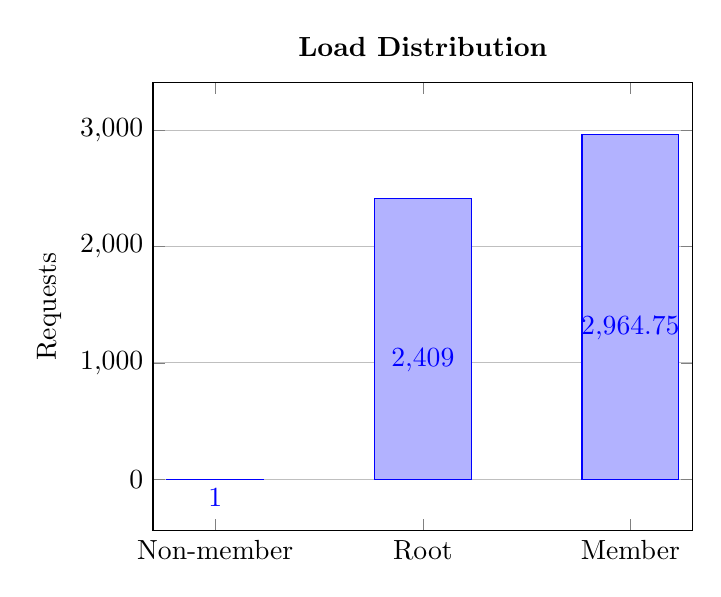
\begin{tikzpicture}
\begin{axis}[
title={\textbf{Load Distribution}},
ybar stacked,
%ymax=50,
ymajorgrids,
bar width=35pt,
%width=250pt,
nodes near coords, 
%nodes near coords={\pgfmathprintnumber\pgfplotspointmeta \%},
nodes near coords align={anchor=north},%Move values in bar
every node near coord/.style={
},
enlargelimits=0.15,
legend style={at={(0.5,-0.20)},
	anchor=north,legend columns=-1},
%width=0.8*\textwidth,
ylabel={Requests},
symbolic x coords={Non-member, Root, Member},
xtick=data,
%legend pos= north east,
%x tick label style={rotate=45,anchor=east},
]
%ethernet
\addplot+[ybar] plot coordinates {(Non-member,1) (Root,2409) 
	(Member,2964.75) };
%\legend{\strut Ethernet}
\end{axis}
\end{tikzpicture}
\caption{Results for load distribution} \label{fig:loaddistribution}
\end{figure}

We discovered that even though the root is loaded with the join requests, the root saves some load, not having to receive its own messages, when forwarding messages. Whereas all the rest of the members also have to receive their own messages during forward.

\section{Message Delivery Latency}
Another goal was to be able to replace existing solutions and therefore it is important that SeriChat is fast and responsive. 
This experiment is intended to measure the latency between the time a root receives a message and the time when this message is received by all the members. 

The experiment was repeated three times using respectively 15, 25, and 80 nodes running the SeriChat prototype. 

The results from the message delivery experiment are, as illustrated in \autoref{fig:messagelatency}. Having in mind that a typical group chat won't have more than 80 members at a maximum, so a latency of 511 ms for a group with 80 member is not that bad. It should be noticed though that this experiment is made locally on one machine, but if it was to be used in a real distributed system the latency will naturally have been higher than these results.   

% pænt
%normal 10-25 antal i grypper --> 80 er en stor gruppe,  erfraing
%511 ms ikke så lang tid
%experiment made locally
%more latency in real distributed systems offcourse
%
\begin{figure}[!h]
	\centering
	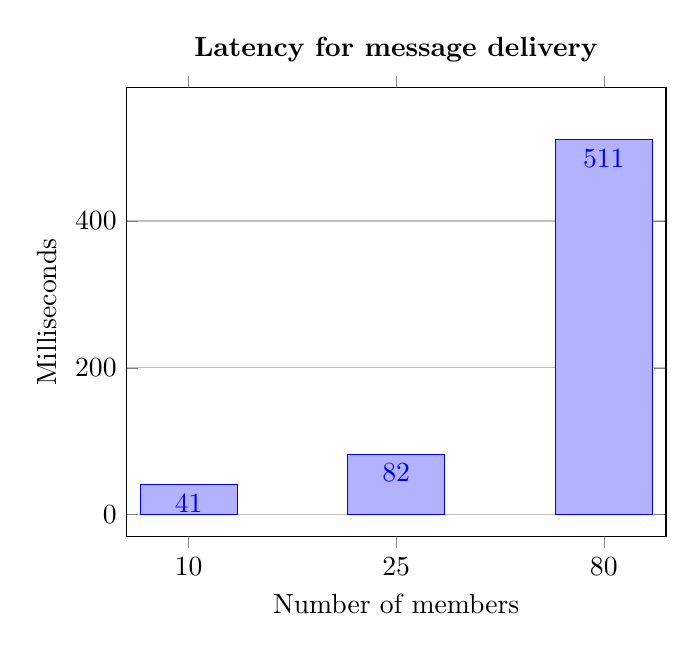
\begin{tikzpicture}
	\begin{axis}[
	title={\textbf{Latency for message delivery}},
	ybar,
	%ymax=50,
	ymajorgrids,
	bar width=35pt,
	%width=250pt,
	nodes near coords, 
	%nodes near coords={\pgfmathprintnumber\pgfplotspointmeta \%},
	nodes near coords align={anchor=north},%Move values in bar
	every node near coord/.style={ 
	},
	enlargelimits=0.15,
	legend style={at={(0.5,-0.20)},
		anchor=north,legend columns=-1},
	%width=0.8*\textwidth,
	ylabel={Milliseconds},
	xlabel={Number of members},
	symbolic x coords={10, 25, 80},
	xtick=data,
	%legend pos= north east,
	%x tick label style={rotate=45,anchor=east},
	]
	%ethernet
	\addplot+[ybar] plot coordinates {(10,41) (25,82) 
		(80,511) };
	
	%\legend{\strut Ethernet}
	\end{axis}
	\end{tikzpicture}
\caption{Results for message delivery latency} \label{fig:messagelatency}
\end{figure}

\chapter{Conclusion}
\label{cha:conclusion}

This, then is the grand summary of what you have accomplished.  You
may well imagine that many readers will read your Introduction, and
then skip to the Conclusion, and if, and only if, those two parts are
interesting, might be tempted to read the rest. A consequence is that
you should ensure that the reader will gain a good overall
understanding of what you have done by reading only the conclusion.
Thus, this is a place to summarise all that has gone before, before
finally concluding on the results of your experiments and the validity
of your hypotheses. It is also important to ensure that the
Introduction (which in all likelihood was written first) still aligns
closely with the conclusions reached.

If you so desire, this is also where you might add a section on Future
Work, where you point in the directions that should be followed to
complete the work you have already accomplished.



%\part{Some Kind of Manual}
%\include{Chapters/Chapter01}
%\cleardoublepage

%\part{The Showcase}
%\include{Chapters/Chapter02}
%\addtocontents{toc}{\protect\clearpage} % <--- just debug stuff, ignore
%\include{Chapters/Chapter03}



%\include{multiToC} % <--- just debug stuff, ignore for your documents
% ********************************************************************
% Backmatter
%*******************************************************
\appendix
%\renewcommand{\thechapter}{\alph{chapter}}
\cleardoublepage
\part{Appendix}
%********************************************************************
% Appendix
%*******************************************************
% If problems with the headers: get headings in appendix etc. right
%\markboth{\spacedlowsmallcaps{Appendix}}{\spacedlowsmallcaps{Appendix}}
\chapter{Guide for Running SeriChat}
To be able to run SeriChat you just have to run this JAR-file through the terminal with the below mentioned steps (it is tested on Linux and Mac OSX).
For each step you have to open a new terminal window.
\graffito{$\leftarrow$ Important read!}

\section{Step-by-Step Guide}
\begin{enumerate}
	\item \textbf{Create the bootstrapping node} 
				\\\texttt{java -jar SeriChat.jar}
	\item \textbf{Create a group by adding: groupowners name, -c (for create) , name of group, and password}
		\\\texttt{ java -jar SeriChat.jar Niels -c AU 123456}
		
	\item \textbf{To join the group: write a name for the new member and replace -c with -j (for join) }
	\\\texttt{java -jar SeriChat.jar Bilal -j AU 123456}
\end{enumerate}

Step 2 and step 3 can be repeated with new names for both the group owners, group members, and new groups.

\section{Example of SeriChat Test Scenario}
Pascal listing below: \autoref{lst:useless}.
\begin{lstlisting}[language=Pascal,frame=tb,caption={A floating example (\texttt{listings} manual)},label=lst:useless]
for i:=maxint downto 0 do
begin
{ do nothing }
end;
\end{lstlisting}
%********************************************************************
% Other Stuff in the Back
%*******************************************************
\cleardoublepage\include{FrontBackmatter/Bibliography}
\cleardoublepage%*******************************************************
% Declaration
%*******************************************************
\refstepcounter{dummy}
\pdfbookmark[0]{Declaration}{declaration}
\chapter*{Declaration}
\thispagestyle{empty}
We hereby declare that this project report entitled: \textbf{\myTitle} is written by us (\myName and \myNametwo) without any third-party.
\bigskip
 
\noindent\textit{\myLocation, \myTime}

\smallskip

\begin{flushright}
    \begin{tabular}{m{5cm}}
        \\ \hline
        \centering\myName \\
    \end{tabular}
\end{flushright}
\begin{flushright}
	\begin{tabular}{m{5cm}}
		\\ \hline
		\centering\myNametwo \\
	\end{tabular}
\end{flushright}

\cleardoublepage\include{FrontBackmatter/Colophon}
% ********************************************************************
% Game Over: Restore, Restart, or Quit?
%*******************************************************
\end{document}
% ********************************************************************
